% Chapter 5
\chapter{Creating Your Own Panels}

\section{How It Works}

\subsection{What You Need}

First you have to read the NanoXML documentation if you need to use XML
in your panel. Secondly, it is necessary that you use the
Javadoc-generated class references. We will just explain here briefly
how to start making your panels.\\

It is a good idea to read the source code of some IzPack panels. They
are usually \textsl{very} small, which makes it easier to understand how
to write your own.\\

\subsection{What You Have To Do}

Extending \IzPack with a panel is quite simple. A panel used with
\IzPack must be a subclass of \texttt{IzPanel}. The \texttt{IzPanel}
class is located in the \texttt{com.izforge.izpack.installer} package
but your panels need to belong to \texttt{com.izforge.izpack.panels}.\\

Things will get a good deal easier if you build IzPack with Jakarta Ant.
Simply add your class in the source tree and add the And directives to
build your own panels. In this way you'll be able to focus on your code
:-)\\

\section{The \texttt{IzPanel} Class}

\subsection{UML Diagram}

\begin{center}
\fbox{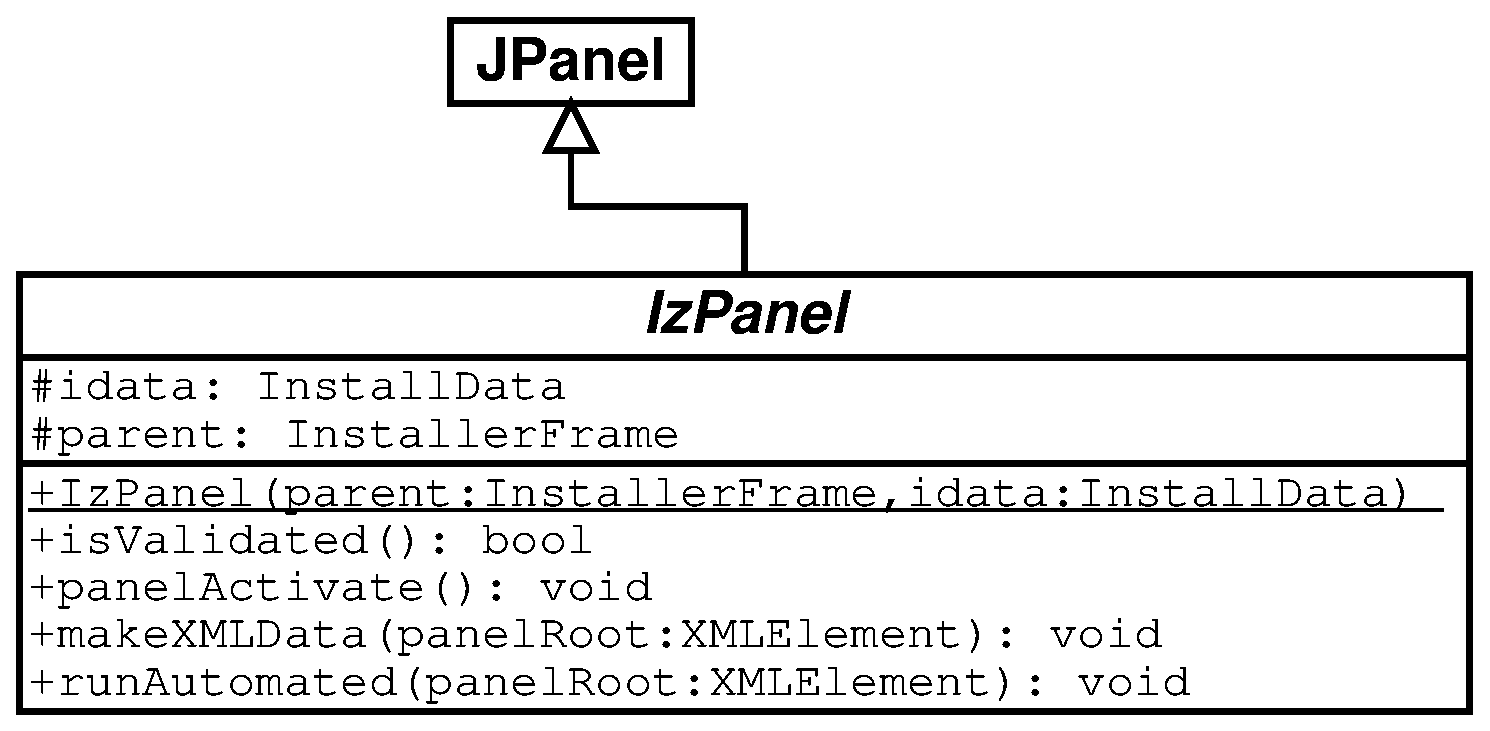
\includegraphics[scale=0.5]{img/ch5-izpanel}}
\end{center}\

\subsection{Description}

The two data members are : the install data (refer to the \texttt{InstallData}
Javadoc reference) and a reference to the parent installer frame.\\

The methods have the following functionality :\\
\begin{itemize}

  \item \textit{(constructor)} : called just after the language
  selection dialog. All the panels are constructed at this time and then
  the installer is shown. So be aware of the fact that the installer
  window is \textbf{not} yet visible when the panel is created. If you
  need to do some work when the window is created, it is in most cases
  better do it in \texttt{panelActivate}.\\

  \item \texttt{isValidated} returns \texttt{true} if the user is
  allowed to go a step further in the installation process. Returning
  \texttt{false} will lock it. For instance the LicencePanel returns
  \texttt{true} only if the user has agreed with the license agreement.
  The default is to return \texttt{true}.\\
  
  \item \texttt{panelActivate} is called when the panel becomes active.
  This is the best place for most initialization tasks. The default is
  to do nothing.\\
  
  \item \texttt{makeXMLData} is called to build the automated installer
  data. The default is to do nothing. \texttt{panelRoot} refers to the
  node in the XML tree where you can save your data. Each panel is given
  a node. You can organize it as you want with the markups you want
  starting from \texttt{panelRoot}. It's that simple.\\
  
  \item \texttt{runAutomated} is called by an automated-mode
  installation. Each panel is called and can do its job by picking the
  data collected during a previous installation as saved in
  \texttt{panelRoot} by \texttt{makeXMLData}.\\

\end{itemize}\
